% !Mode:: "TeX:UTF-8"
\documentclass[newtxmath=true,newgeometry=two,capcenterlast=true,subcapcenterlast=true,openright=true,absupper=true,fontset=windowsnew,type=master]{hithesis}
% 此处选项中不要有空格
%%%%%%%%%%%%%%%%%%%%%%%%%%%%%%%%%%%%%%%%%%%%%%%%%%%%%%%%%%%%%%%%%%%%%%%%%%%%%%%%
% 必填选项
% type=doctor|master|bachelor
%%%%%%%%%%%%%%%%%%%%%%%%%%%%%%%%%%%%%%%%%%%%%%%%%%%%%%%%%%%%%%%%%%%%%%%%%%%%%%%%
% 选填选项(选填选项的缺省值已经尽可能满足了大多数需求,除非明确知道自己有什么
% 需求)
% glue=true|false
% 	含义:由于我工规范中要求字体行距在一个闭区间内,这个选项为true表示tex自
% 	动选择,为false表示区间内一个最接近版心要求行数的要求的默认值,缺省值为
% 	false。
% tocfour=true|false
% 	含义:是否添加第四级目录,只对本科文科个别要求四级目录有效,缺省值为
% 	false
% fontset=siyuan|windowsnew|windowsold
% 	含义:注意这个选项视为了解决特殊问题而设置,比如用有些发行版本的linux排
% 	版时可能(大多数发行版不会)会遇到的字体无法载入的问题,或者字体载入之
% 	后出现无法复制的问题以及想要解决排版如 biang biang 面的 biang 这类中易
% 	宋体无法识别的汉字的问题。没有特殊的需要不推荐使用这个选项。
%
% 	如果是安装了 windowns 字体的 linux 系统,可以填写windowsnew(win vista
% 	以后 的字体)或 windowsold(vista 以前)或者想用思源宋体并且是已经安装
% 	了思源宋体的任何系统,填写siyuan选项。缺省值为空,自动识别系统并匹配字体
% 	。模板版中给出的思源字体定义文件定义的思源字体的版本是Adobe版,其他字体
% 	是windowsnew字体。
% tocblank=true|false
% 	含义:目录中第一章之前,是否加一行空白。缺省值为true。
% chapterhang=true|false
% 	含义:目录的章标题是否悬挂居中,规范中要求章标题少于15字,所以这个选项
% 	有无没什么用,除了特殊需求。缺省值为true。
% fulltime=true|false
% 	含义:是否全日制,缺省值为true。非全日制如同等学力等,要在cover中设置类
% 	型,封面中不同格式
% subtitle=true|false
% 	含义:论文题目是否含有副标题,缺省值为false,如果有要在cover中设置副标
% 	题内容,封面中显示。
% newgeometry=one|two
% 	含义:规范中的自相矛盾之处,版芯是否包含页眉页脚,旧方法是按照包含页眉
% 	页脚来设置。该选项是多选选项,如果没有这个选项,缺省值是旧模板的版芯设
% 	置方法,如果设置该选项one或two,分别对应两种页眉页码对应版芯线的相对位
% 	置。第一种是严格按照规范要求,难看。第二种微调了页眉页码位置,好一点。
% debug=true|false
% 	含义:是否显示版芯框和行号,用来调试。默认否。
% openright=true|false
% 	含义:博士论文是否要求章节首页必须在奇数页,此选项不在规范要求中,按个
% 	人喜好自行决定。 默认否。注意,窝工的默认情况是打印版博士论文要求右翻页
% 	,电子版要求非右翻页且无空白页。如果想DIY(或身不由己DIY)在什么地方右
% 	翻页,将这个选项设置为false,然后在目标位置添加`\cleardoublepage`命令即
% 	可。
% capcenterlast=true|false
% 	含义:图题、表题最后一行是否居中对齐(我工规范要求居中,但不要求居中对
% 	齐),此选项不在规范要求中,按个人喜好自行决定。默认否。
% subcapcenterlast=true|false
% 	含义:子图图题最后一行是否居中对齐(我工规范要求居中,但不要求居中对齐
% 	),此选项不在规范要求中,按个人喜好自行决定。默认否。
% absupper=true|false
%       含义:中文目录中的英文索引在中文目录中的大小写样式歧义,在规范中要求首
%       字母大写,在work样例中是全大写。该选项控制是否全大写。默认否。
% bsmainpagenumberline=true|false
%       含义:由于本科生论文官方模板的页码和页眉格式混乱,提供这个选项自定义设
%       置是否在正文中显示页码横线,默认否。
% bsfrontpagenumberline=true|false
%       含义:由于本科生论文官方模板的页码和页眉格式混乱,提供这个选项自定义设
%       置是否在前文中显示页码横线,默认否。
% bsheadrule=true|false
%       含义:由于本科生论文官方模板的页码和页眉格式混乱,提供这个选项自定义设
%       置是否显示页眉横线,默认显示。
% splitbibitem=true|false
%       含义:参考文献每一个条目内能不能断页,应广大刀客要求添加。默认否。
% newtxmath=true|false
%       含义:数学字体是否使用新罗马。默认是。
%%%%%%%%%%%%%%%%%%%%%%%%%%%%%%%%%%%%%%%%%%%%%%%%%%%%%%%%%%%%%%%%%%%%%%%%%%%%%%%%

\usepackage{hithesis}
\usepackage[ruled]{algorithm2e}
\graphicspath{{figures/}}

\begin{document}

\frontmatter
% !Mode:: "TeX:UTF-8"

\hitsetup{
  %******************************
  % 注意:
  %   1. 配置里面不要出现空行
  %   2. 不需要的配置信息可以删除
  %******************************
  %
  %=====
  % 秘级
  %=====
  statesecrets={公开},
  natclassifiedindex={TM301.2},
  intclassifiedindex={62-5},
  %
  %=========
  % 中文信息
  %=========
  ctitleone={局部多孔质气体静压},%本科生封面使用
  ctitletwo={轴承关键技术的研究},%本科生封面使用
  ctitlecover={面向自动驾驶系统测试用例生成的对抗生成网络和图像风格转换技术的实证研究},%放在封面中使用,自由断行
  ctitle={面向自动驾驶系统测试用例生成的对抗生成网络和图像风格转换技术的实证研究},%放在原创性声明中使用
  csubtitle={一条副标题}, %一般情况没有,可以注释掉
  cxueke={工学},
  csubject={计算机技术},
  caffil={创新创业学院},
  cauthor={闫施违},
  csupervisor={张煜群},
  % 日期自动使用当前时间,若需指定按如下方式修改:
  %cdate={超新星纪元},
  cstudentid={11749199},
  cstudenttype={同等学力人员}, %非全日制教育申请学位者
  %(同等学力人员)、(工程硕士)、(工商管理硕士)、
  %(高级管理人员工商管理硕士)、(公共管理硕士)、(中职教师)、(高校教师)等
  %
  %
  %=========
  % 英文信息
  %=========
  etitle={An empirical study of GANs and Neural Style Transfers for test case generation in autonomous driving system},
  esubtitle={This is the sub title},
  exueke={Engineering},
  esubject={Computer Technology},
  eaffil={\emultiline[t]{School of Innovation and Entrepreneurship}},
  eauthor={Shiwei Yan},
  esupervisor={Professor Yuqun Zhang},
  % 日期自动生成,若需指定按如下方式修改:
  edate={December, 2017},
  estudenttype={Master of Art},
  %
  % 关键词用“英文逗号”分割
  ckeywords={自动驾驶, 深度学习, 对抗生成网络, 图像风格转换},
  ekeywords={autonomous driving, deep learning, GAN, neural style transer},
}

\begin{cabstract}

近年来,得益于深度学习的发展,自动驾驶的研究与开发也取得了巨大的突破。国内外的许多公司都开发了自己的自动驾驶系统框架,譬如Google公司的Waymo,Baidu公司的Apollo和Tesla公司研制的Autopilot,其中最为人熟知的Autopilot已经成功的部署运行在了现实商用的Tesla轿车中。

尽管各大公司都标榜如今的自动驾驶系统安全性能已经足够高,但是近一两年发生的几起自动驾驶车祸引起了人们对于自动驾驶系统安全性能的关注,下左图是于2018年3月23号,发生在美国加州山景城高速公路上的一起车祸,事后事故分析指出由于Autopilot未能识别灰色公路背景下的白色防护栏从而导致的车祸的发生。同样的右图也是由于Uber公司研制的自动驾驶系统的误判,于2017年发生在美国亚利桑那州天普城的一起车祸。

\begin{figure}[h]
  \centering
  \subfigure[车祸1]{
          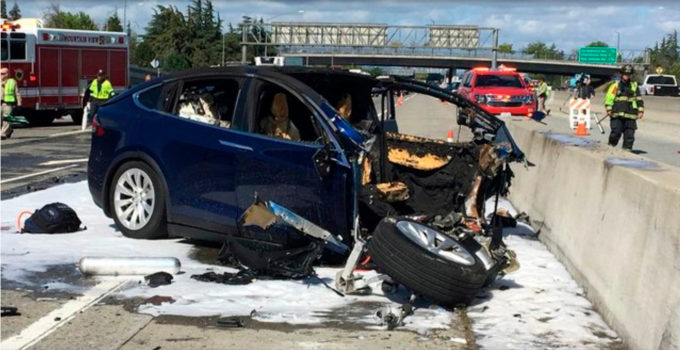
\includegraphics[width=0.45\textwidth, height=4cm]{crash_t}
  }
  \subfigure[车祸2]{
          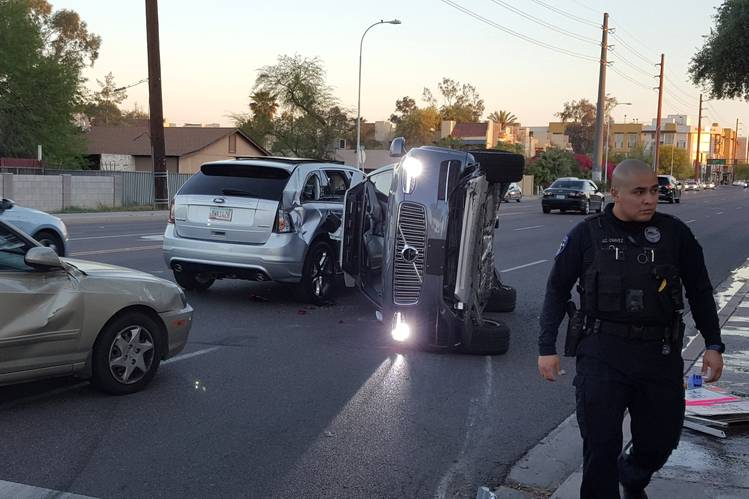
\includegraphics[width=0.45\textwidth, height=4cm]{crash_u}
  }
  \caption{crashs}
\end{figure}

除了上述之外,近年来还陆续有自动驾驶相关的车祸发生,以上种种都表明当前的自动驾驶的安全性能并没有人们认为的那么高。为了提升自动驾驶系统的安全等级,工业界和学术界都在此做了很多研究,于2017年学术界在此领域先后发表了2篇重要的文章,DeepXplore\cite{DeepXplore}和DeepTest\cite{DeepTest},DeepXplore提出了一套深度学习系统测试用例自动生成的框架。DeepTest延伸了DeepXplore的工作并将前者的方法成功的运用到了自动驾驶系统测试用例,即驾驶路况场景图,生成中,两者的工作都以现实的自动驾驶框架为测试对象,成功生成除了很多自动驾驶系统会误判的测试用例,这对提升自动驾驶系统的安全性能有着重大意义。

基于DeepXplore和DeepTest的工作,我所在的实验室提出了DeepRoad\cite{DeepRoad},它借助对抗生成网络\cite{GAN}中的UNIT\cite{UNIT}框架提升了生成的自动驾驶测试用例,即驾驶场景图片的质量。在本论文中,我们做了针对现有的深度学习技术,主要包含对抗生成网络和图像风格转换技术,做了大量的实证研究,以探讨哪个已有的深度学习技术对于自动驾驶测试用例生成,即驾驶场景图片的合成,是最有效的。

本工作希望能为之后的自动驾驶系统测试人员在选择驾驶场景图片测试用例自动生成的框架选择上可以给出一些有价值的建议。

\end{cabstract}

\begin{eabstract}
  In recent years, thanks to the development of deep learning, the research and development of autonomous driving has also made great breakthroughs. Many companies at home and abroad have developed their own autopilot system frameworks, such as Google's Waymo, Baidu's Apollo and Tesla's Autopilot. The most well-known Autopilot has been successfully deployed in real-life commercial Tesla sedan. in.

  Although major companies have advertised that the safety of today's autopilot systems is high enough, several autopilot accidents in the past year or two have caused concern about the safety performance of autopilot systems. The picture on the left is in March 2018. On the 23rd, a car accident occurred on the Highway in Mountain View, California, USA. The post-accident analysis pointed out that the car accident caused the failure of Autopilot to identify the white fence on the gray road background. The same right picture is also due to a misjudgment of the autopilot system developed by Uber, which occurred in 2017 in a car accident in Temple City, Arizona, USA.

  In addition to the above, there have been autopilot-related car accidents in recent years, all of which indicate that the current safety of autonomous driving is not as high as people think. In order to improve the safety level of the automatic driving system, the industry and academia have done a lot of research here. In 2017, the academic community has published two important articles in this field, DeepXplore\cite{DeepXplore} and DeepTest\cite{ DeepTest}, DeepXplore proposes a framework for automatic generation of test cases for deep learning systems. DeepTest extends DeepXplore's work and successfully applies the former method to the autopilot system test case, that is, the driving road scene graph, the generation, both work are based on the actual auto-driving framework as the test object, successfully generated in addition to many automatic Test cases that are misjudged by the driving system are of great significance for improving the safety performance of the autonomous driving system.

  Based on the work of DeepXplore and DeepTest, my lab has proposed DeepRoad\cite{DeepRoad}, which enhances the generated autopilot test case by using the UNIT\cite{UNIT} framework in the anti-generation network \cite{GAN}. The quality of the driving scene picture. In this paper, we have done a lot of empirical research on existing deep learning techniques, including anti-generation network and image style conversion techniques, to explore which existing deep learning techniques are used for autopilot test case generation. That is, the synthesis of the driving scene picture is the most effective.

  This work hopes to give some valuable suggestions for the subsequent autopilot system testers to choose the framework of the auto-generated framework for driving scene picture test cases.
\end{eabstract}

% word count ~ 1000
 % 封面
\makecover
\input{front/denotation}%物理量名称表,符合规范为主,有要求添加
%\cleardoublepage  自定义在什么位置进行右翻页
\tableofcontents    % 中文目录
%\cleardoublepage  自定义在什么位置进行右翻页
\tableofengcontents % 英文目录,硕本不要求

\mainmatter
%\linenumbers %debug 选项
%\layout %debug 选项
%\floatdiagram %debug 选项
%\begin{figure} %debug 选项
%\currentfloat %debug 选项
%\tryintextsep{\intextsep} %debug 选项
%\trytopfigrule{0.5pt} %debug 选项
%\trybotfigrule{1pt} %debug 选项
%\setlayoutscale{0.9} %debug 选项
%\floatdesign %debug 选项
%\caption{Float layout with rules}\label{fig:fludf} %debug 选项
%\end{figure} %debug 选项
% !Mode:: "TeX:UTF-8"

\chapter{背景}[Background]

虽然目前很多公司都开发了自己的自动驾驶系统,但其使用的技术几乎都是基于计算机视觉,目标检测,目标识别等深度学习、机器学习技术。因此,针对自动驾驶系统的测试技术也是源于深度学习系统的测试技术。其中,在基于深度神经网络的自动驾驶系统中,其神经网络模型将被汽车的各种传感器(雷达、摄像头等)接收到的数据作为输入,经过神经元的运算处理后输出各种驾驶行为(方向盘拐角、刹车信号,速度控制信号等)。下图\ref{as_example}展示了一个机遇卷积神经网络的自动驾驶系统例子,这个系统由输入(摄像头拍摄的图像)、输出层(方向盘拐角)和中间的隐藏层组成。本章主要讲述传统的深度学习测试技术以及目前学术界比较推崇的自动测试技术。

\begin{figure}[h]
    \centering
    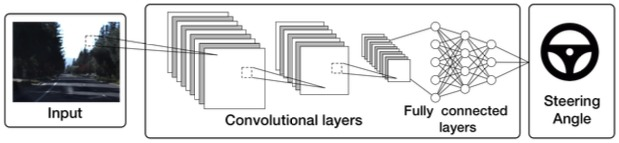
\includegraphics[width=0.8\textwidth]{as_example}
    \caption{基于卷积神经网络的自动驾驶系统\cite{DeepRoad}}
    \label{as_example}
\end{figure}

\section{传统的深度学习系统测试技术}[The traditional testing technology of DNN]

深度学习技术是一种通过研究同类大量数据的表征,对未知新数据的特征进行推测的一门技术。在其行使职能,即预测新数据特征前,必须要学习大量同类的数据,即模型训练。模型训练完成后为了提前检测模型的准确性,会在之前的训练数据集中保留一部分数据,作为训练结束后的模型的测试数据集,使其在未被学习过的测试数据集上进行预测,最后以测试数据集上的准确性作为训练好的模型的精准度。目前学术界公认理想的训练数据集与测试数据集占比分别为70\%和30\%。

% TODO 可扩展

数据集的具体数量跟模型处理的具体问题相关,一般来说,处理的问题越复杂,即数据的特征越多,需要的数据量也就越多,比如比较出名的ImageNet\cite{ImageNet}比赛,公开可用的数据集多达1500万张由人工标注的图片数据。深度学习技术对已有数据特征拟合的本质和其训练测试的过程导致其对数据量的严重依赖,传统的深度学习测试需要大量的人工收集、标注数据,着极度的增加了其中的人力成本。除此之外,传统的通过人工收集数据的方式有严重的缺点,即收集到的数据无法保证覆盖到了所有可能的极端场景,以自动驾驶测试数据集为例,人工收集的数据集一般是车载记录仪记录的道路驾驶视频图片,但一般大雨、大雪等极端天气场景数据很少也很难收集,这就给相应的极端场景自动驾驶系统测试带来了不确定性。

\section{DeepXplore、DeepTest和DeepRoad}[DeepXplore DeepTest and DeepRoad]

针对上诉问题,DeepXplore和DeepTest提出了深度学习系统测试用例自动生成系统来缓解深度学习系统对于数据量的依赖。

\subsection{DeepXplore}[DeepXplore]
DeepXplore首先指出了深度学习系统与传统的软件开发系统的不同:传统软件的开发人员直接指定软件系统的逻辑,然而深度学习则是从数据特征中“学习、推到”它们的运行规则,甚至对于深度学习系统的开发人员来说,他们都不一定清楚训练好的深度学习模型的确切运行逻辑。因此DeepXplore
不是直接寻找深度学习系统中的逻辑错误,而是通过自动产生、寻找一些能使多个同类深度学习系统做出不同行为判断的测试用例,然后并将这些找到的测试用例放回原训练数据集里重新训练模型,试图修正之前错误的行为

除了将使不同的DNN系统做出不同预测行为为目标外,DeepXplore也借鉴了传统软件测试技术中的代码覆盖率的概念,为了使得尽可能测试整个DNN系统,DeepXplore引入了神经元覆盖率的概念,即测试用例测试过程中,在整个深度学习系统中,被“激活”,即输出值超过了某个阀值,的神经元的个数占整个网络结构神经元总数的占比。与代码覆盖率类似,我们期望神经元覆盖率越高越好。

DeepXplore以神经元覆盖率和使得不同DNN系统输出不一致为目标,将在原始测试用例上的修改抽象成为一个优化算法,使用梯度上升算法,最后自动生成一些使得被测的DNN系统得到不同的预测值,且各个DNN系统的神经元覆盖率很高的测试用例,下图\ref{xplore-wf}是DeepXplore的工作原理图。

\begin{figure}[h]
    \centering
    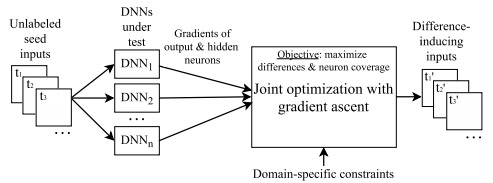
\includegraphics[width=0.8\textwidth]{xplore-wf}
    \caption{DeepXplore工作原理图\cite[图~5]{DeepXplore}}
    \label{xplore-wf}
\end{figure}

\subsection{DeepTest}[DeepTest]

DeepTest基于DeepXplore的工作,提出了一套专门针对自动驾驶系统,能够自动检测出错误行为的测试系统。发生在自动驾驶系统上的车祸大部分都是发生在一些罕见的路况场景下,而传统的自动驾驶检测测试技术几乎是完全依赖大量的罕见路况场景图片的人工收集与标注,这不仅包含了大量的人工成本,重要的是人工收集的数据无法保证能够覆盖度到了所有的极端场景数据。这些极端场景就好像是传统软件中的bug,但是这些bug一旦被检测到,就可能通过把这些导致错误的输入重新放入训练集,同时改变一下模型的结构和参数来修复。DeepTest正是通过以上的思路来设计的一套自动测试系统。

\begin{algorithm}[h]
    \small
    \SetAlgoLined
    \SetKwInOut{Input}{Input}
    \SetKwInOut{Output}{Output}
    \SetKwInOut{Variable}{Variable}

    \Input{变换Transformations T, 种子图像Seed Images I}
    \Output{合成的测试数据图像}
    \Variable{S: 存储新合成图像的栈; Tqueue: 存储变换的队列}

    push all seed imgs to Stack S; 所有种子图片入栈\;
    $genTests = \varnothing$\;
    \While{S is not empty}{
        img = S.pop()\;
        $Tqueue = \varnothing$\;
        numFailedTries = 0 \;
        \While{$numFailedTries \leq maxFailedTries$}{
            \eIf{$Tqueue\ is\ not\ empty$}{
                T1 = Tqueue.deque()
            }{
                Randomly pick transformations T1 from T
            }
            Randomly pick parameter P1 for T1\;
            Randomly pick transformation T2 from T\;
            Randomly pick parameter P2 from T2\;
            newImage = ApplyTransforms(image, T1, P1m T2, P2)\;
            \eIf{covInc(newiamge)}{
                Tqueue.enqueue(T1)
                Tqueue.enqueue(T2)
                UpdateCoverage()
                $genTests=genTests \cup newiamge S.push(newImaghe)$
            }{
                $numFailedTries=numFailed++$
            }
        }
    }
    return genTests
    \caption{混合变换优化算法\cite{DeepTest}}
    \label{alg1}
\end{algorithm}

具体的实现上,DeepTest依旧借用DeepXplore提出的神经元覆盖率的概念,使用位移、拉伸、仿射以及直接修改像素的透明度等基本的图形变换的手段来合成新的驾驶图像,文章里提到合成后的数据能使原DNN系统的神经元覆盖率提升100\%\cite{DeepTest},并以提升神经元覆盖率为目标,给出了一个优化算法\ref{alg1},以获得最佳的图像混合变换,最后DeepTest在利用这些合成的新数据重新训练自动驾驶模型来提高模型对于极端场景的鲁棒性。

\subsection{DeepRoad}[DeepRoad]

尽管DeepTest已经提出了一个较为完善的自动驾驶系统测试方案,以相对便宜和简洁的方法,利用大量的原始和合成出来的驾驶场景图片成功地检测出了许多自动驾驶系统前后不一致的驾驶行为,但它有一个很严重的缺陷:DeepTest用来合成图片的技术很难合成一些能够精确反映现实驾驶场景的图片,并且现实驾驶场景的图片也很难由一些基础的仿射、位移变换模拟合成出来,其用来模拟雨天、雾天的场景的技术仅仅是在原始图层上添加一层额外的图层,如下图\ref{deeptest_effect}所示,对于雾天,DeepTest仅仅是加了一层白色的图层,对于雨天,加了一层线条层。很明显这些合成图离现实中真实的驾驶场景有较大的差别。从另一个角度来说,即时用这些图检测出了自动驾驶系统错误的驾驶行为也很难有说服力,因为这些“出错”的场景在现实中根本不会出现。其实很多可能的真实的驾驶场景根本不能用一些简单的图像处理技术来模拟合成。

\begin{figure}[h]
    \centering
    \subfigure[DeepTest]{
        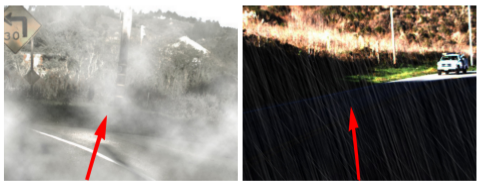
\includegraphics[width = 0.7\textwidth]{deeptest_effect}
    }
    \subfigure[DeepRoad]{
        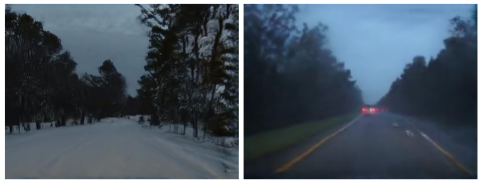
\includegraphics[width = 0.7\textwidth]{deeproad_effect}
    }
    \label{deeptest_effect}
    \caption{天气场景合成效果图比较}
\end{figure}

为了能够自动地合成大量真实的驾驶场景图片,DeepRoad提出了一个半监督合成的框架,抛弃了DeepTest用到的简单的图像处理技术来合成图像,采用深度学习对抗生成网络的技术来合成相对较真实的驾驶场景图片,上图\ref{deeptest_effect}为DeepTest合成图和DeepRoad使用对抗生成网络中UNIT\cite{UNIT}框架合成图的效果对比。可以清楚的看到使用UNIT技术合成的效果比较好的驾驶场景图已经与真实场景很接近了。下图\ref{deeproad_wf}展示了DeepRoad框架的整体流程。 

\begin{figure}[h]
    \centering
    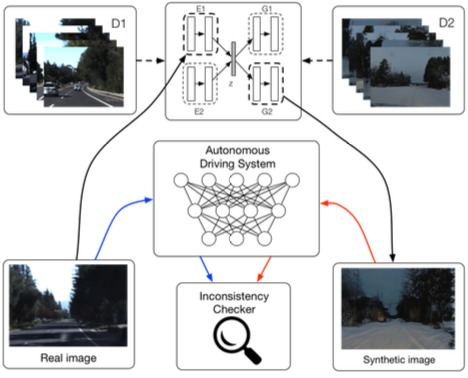
\includegraphics[width=0.75\textwidth]{deeproad_wf}
    \caption{DeepRoad框架流程图\cite{DeepRoad}}
    \label{deeproad_wf}
\end{figure}

DeepRoad将两种天气情况下的图片作为训练输入数据集,训练无监督对抗生成网络UNIT\cite{UNIT}框架,然后利用训练好的UNIT框架对未知新的输入数据进行转换合成,最后测试自动驾驶系统对使用UNIT进行转换后的图片做出的驾驶行为与未转换之前的原始图片的驾驶行为是否一致。

\section{其他的图像转换技术}[Other Image Transformation Technologies]

DeepRoad提出的将深度学习技术运用到自动驾驶系统测试用例合成,并设计的一套自动测试的框架在检测自动驾驶系统的稳定性和鲁棒性上,在其实验检测出了大量的现实自动驾驶系统有误的驾驶行为的结果\cite{DeepRoad}上看是有效的。其相对前人的工作DeepTest主要的改进是将测试用例的合成技术,即驾驶场景的图像转换技术,由原有的基本的图像变换换成了深度学习中的对抗生成网络技术。我们在利用UNIT合成驾驶场景图的实验过程中发现,虽然有效果比较好的合成图,但其占总的合成图的比例很小,1万张结果图中比较真实的图像大约有30多张,大部分的结果图如下,可以看到效果比较差,我们分析了效果比较差的原因主要是使用的训练数据集是由我们从Youtube上爬取的视频制作的数据图像,与UNIT官方使用的NVIDIA公司提供的闭源数据集相差比较大导致。

但其实目前学术界和工业界已经提出的能够进行不同天气场景图像转换的深度学习技术有很多,我们进行了调研,发现主要有两大类:对抗生成网络和图像风格转换(Neural Style Transfer)。我们对DeepRoad进行的实验也表明在得不到理想的训练数据集的情况下利用UNIT进行图像转换的实验结果是不理想的,那么可否将UNIT更换为其他的能够进行图像转换的深度学习技术?哪一种技术的实现效果是最好的?如何评价各种图像转换技术在合成驾驶场景图上的好坏?哪一种技术的训练成本和实现成本是最小的?针对以上问题,我们对现有的能够实现图像风格转换的深度学习技术展开实证研究,希望能够找到答案,最终可以为以后的自动驾驶系统测试人员在选择驾驶场景图片测试用例的合成技术框架上提供一些有帮助的建议。

% TODO UNIT图像

% word count ~ 3450

\chapter{实验}[Methodology]

% metrics -> intro of every gan and experiment, show results

为了尽可能地对所有能够实现图像风格变换的深度学习框架进行试验结果对比,我们首先调研了目前对图片合成图质量的量化评价指标,结合测试人员在实际测试过程中的各种成本以及实验细节,我们总结出了了3个指标: \textit{Fre ́chet Inception Distance(FID)}\cite{FID},模型训练时长以及自动驾驶系统对于前后合成图行为判断方向盘拐角差。

\section{评价指标}[Metrics]

对于图像驾驶场景合成图的质量好坏,最直观也是最直接的方式就是比较合成图的视觉效果,但这种人为的评判是主观且十分容易误判的。为了能够客观、量化的比较各个DNN框架合成的驾驶场景图的好坏,学术界提出了两个指标:\textit{Inception Score(IS)}\cite{IS}和\textit{Fre ́chet Inception Distance(FID)}\cite{FID}。

\textbf{Inception Score(IS).\cite{IS}}\quad IS评价合成图片质量是基于以下两点:(i) 包含有意义的物体图像的条件标记分布应该具有较低的熵(entropy)和(ii) 图像的多样性应该较高,进而边缘分布$\int_z p(y|x=G(z))dz$应该有较高的熵。
将以上两点汇总成一个评分,
\begin{center}
    $IS(G)=\exp{(E_{x\sim G}[d_{KL}(p(y|x), p(y)])}$
\end{center}
IS的作者用ImageNet\cite{ImageNet}的数据训练了一个分类器,最终实验结果反映IS的分数与人工标注评价正相关。

\textbf{Fre ́chet Inception Distance(FID).\cite{FID}}\quad FID提出了另一个评价方法,它首先将所有的合成图片放入一个特征空间,然后将该空间视为一个多元高斯分布,分别计算合成图和真实图的均值与方差,将两者高斯分布的Fre ́chet距离来量化真实图与合成图之间的距离,进而作为对合成图的评价:
\begin{center}
    $FID(x,g)=||\mu_x-\mu_g||_2^2+Tr(\sum_x + \sum_g - 2(\sum_x\sum_g)^{\frac{1}{2}})$
\end{center}
这里的$(\mu_x,\sum_x)$和$(\mu_g,\sum_g)$分别是数据分布和模型分布的均值和方差。FID的作者发现FID值与人类对合成图像的判断一直,并且较IS\cite{IS}鲁棒性更强。相对于IS,FID还能检测出不同类之间的区别,即如果每一种类别值产生合成一张图片,则很有可能获得比较高的IS分数,但对应的FID值却很低。基于以上几点,我们选用FID值而不选择IS值作为我们后面实验评价合成图片质量的评价指标之一。

\textbf{模型训练时长.}\quad 除了直接比较合成图片质量的好坏,在实际的自动驾驶系统测试过程中,我们还必须考虑到模型的训练时长。在选择理想的图片合成框架时,除了最终合成图片质量的好坏,我们还希望模型的训练时间成本尽可能的小,不同的模型根据不同的训练数据集大小,最终的训练时长也相差越大,比如本章后面会提到的UNIT\cite{UNIT}基于Udacity自动驾驶数据集\cite{udacity_dataset}和大约3000张驾驶场景图片,训练50万次时长大约一周左右。而对于一些图像风格转换(Neural Style Transfer)模型来说,训练时长却只要几个小时,虽然最后合成图的质量不如UNIT,但我们希望把这些数据都统计出来,具体的取舍留给实际最终的测试人员自己选择。 

\textbf{方向盘拐角差.}\quad 有了合成图质量的量化指标,模型的训练时间成本比较,最后我们还希望直观地看到合成图相比原始图对于自动驾驶系统行为判断(方向盘拐角信号)的影响。理想情况下,只变换驾驶场景图片的风格,比如晴天的路况转换为夜晚、雨天或者阴天的路况,自动驾驶系统对于大部分的转换后的图像的行为判断,即输出的方向盘拐角信号,与原始的驾驶路况图片做出的行为判断应该几乎一致,或者差别不大。实验中我们对两者的信号,即拐角差设置了一个阈值$\alpha=5^{\circ}$,我们希望小于阈值的图片占比越小越小,最后我们以两者之间拐角差的方差作为该指标的量化数据。

综上述,在后面的实验中,我们将统计所有实验模型的\textbf{FID值}、\textbf{模型训练时长}和\textbf{方向盘拐角差}3个指标。

% wc ~ 1400

\section{模型的筛选与实验}[Model Filting and Experiments]

基于DeepRoad的工作,我们首先选择实验的DNN模型大类是对抗生成网络\cite{GAN},因为其生成仿照数据的功能契合我们对于合成驾驶场景图片的需求,下面简单的介绍一下对抗生成网络的背景以及选择的对应模型。

\subsection{对抗生成网络大类}[Generative Adversarial Network Class]

对抗生成网络\cite{GAN}首先由Ian J. Goodfellow等人提出,它的本质是模拟真实数据源的概率分布。其基本框架有两个神经网络组成:生成模型网络和判别模型网络,其中判别模型负责学习区分数据是否来自真实数据分布,而生成模型可以想象成一个制造伪币的团伙,试图产生能够通过货币监测的钞票,判别模型正是这个对抗游戏中的警察,试图甄别出货币中的假钞。整个对抗生成网络模型的训练过程就是对抗模型和生成模型的训练竞赛,整个训练过程直到判别模型再也区分不出数据是来自真实数据分布还是生成模型伪造的数据为止。

训练过程中,对抗模型一般使用向后传播算法,而判别模型一般使用向前传播算法。其中判别模型为了通过数据$x$学习生成器的数据分布$p_g$,可以基于输入的噪声数据定义一个先验概率$p_z(z)$,然后将整个数据空间表示为$G(Z;\theta_g)$,这里的$G$是一个参数为$\theta$的多层神经网络可微函数。再定义一个输出为一个单向量的多层神经元网络$D(x;\theta_d)$,其中$D(x)$表示数据$x$来自真实数据而非$p_g$的概率。我们训练$D$直到我们对所有数据正确标记其是否来自判别器的概率最大为止。同时也训练$G$来最小化$\log(1-D(G(z)))$。上述可总结成下面的公式:
\begin{equation}
    \label{eq:gan}
    \min_G\max_DV(D,G)=\xi_{x\sim p_{data}(x)}[\log D(x)]+\xi_{z\sim p_z(z)}[\log(1-D(z))]
\end{equation}
实际训练过程中,等式\eqref{eq:gan}中的生成器$G$可能会出现梯度消失的问题,但由于本文章不是对对抗生成网络算法的研究,所以就不在此展开了。

为了对目前所有的对抗生成网络技术能有一个综合的认识,我们主要参考了文献\cite{gan-survey},跟据文献中的分类,依次对每种类型中比较典型的框架进行了实验与数据总结统计。实验过程中为了保持尽量跟框架作者实现的效果性能一致,我们只选取了提供了源代码的框架进行了实验。

% TODO: confirm this
\textbf{统一说明},本文后续所有的实验均是在64位Ubuntu操作系统,8核1080ti-GPU硬件环境下进行的。

\subsubsection{DCGAN}[DCGAN]

\textbf{DCGAN.}\cite{dcgan}\quad 是一个深度卷积对抗生成网络,其生成器和判别器使用的是限制卷积网络,主要的架构特点有:(1)用多步卷积和分布卷积层代替了所有的池化层(pooling layer);(2)使用了批量统一化层(batch normalization layer);(3)去掉了所有的全连接层;(4)在生成器中,使用$\tan{h}$作为输出层的激活函数,ReLU函数作为其它层的激活函数;(5)判别器中,所有层的激活函数都使用LeakyReLU函数。

虽然DCGAN的作者将其运用在人脸合成与转换上相当成功,但我们后来将其训练集换成了Udacity的自动驾驶路况数据集以及youtube上爬取的数据,实验结果样本图如下图\ref{dcgan_example}所示,效果却不理想。

\begin{figure}[h]
    \centering
    \subfigure[DCGAN在人脸图像合成的效果样例图]{
        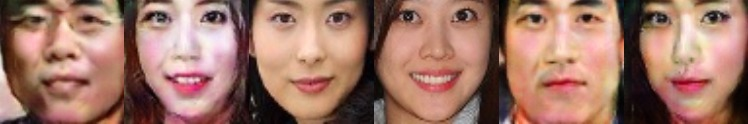
\includegraphics[width=0.75\textwidth]{dcgan_example}
    }
    % TODO: add dcgan result imgs.
    \caption{}
    \label{dcgan_example}
\end{figure}

实验代码使用的是\cite{dcgan}论文中给出的代码,其中主要参数配置如下

% TODO: confirm
\begin{lstlisting}[basicstyle=\small]
    --bathSize     200          // 批量实验数据大小
    --imageSize    180, 320     // 设置图像尺寸大小
    --nz           20           // z向量
    --niter        10000        // 训练的次数
    --lr           0.0002       // Learning rate
    --cuda                      // 在cuda库上训练
\end{lstlisting}

由于DCGAN在驾驶路况图片上的合成效果很差,于是我们放弃了对该框架进一步的实验结果数据统计与总结。

% wc ~ 1200

\subsubsection{CycleGAN}[CycleGAN]

\textbf{CycleGAN.}\cite{CycleGAN}\quad 该模型的本质是学习不同图片类(比如晴天和雨天)的数据分布映射函数。给定两个不同类的数据集$X$和$Y$以及训练样本集$\{x_i\}_{x=1}^N, \{y_j\}_{j=1}^M$,其中$x_i\in X, y_j\in Y$。将数据分布记为$x\sim p_{data}(x), y\sim p_{data}(y)$。如图\ref{cyclegan_1}所示,CycleGAN包含两个映射函数$G: X\to Y$和$F: Y\to X$,其次,CycleGAN还引进了两个判别器$D_X$和$D_Y$,其中$D_X$的目标是区分图像集$\{x\}$和转换的图像集$\{F(y)\}$,同样的,$D_Y$的目标是区分图像集$\{y\}$和$\{G(x)\}$。最终模型的训练目标是得到两个损失函数:(i)对抗损失函数,可以将合成的图像数据分布匹配对应到目标类的数据分布上;(ii)循环一致损失函数,阻止之前学习到的两个映射函数$G$和$F$彼此相矛盾。

\begin{figure}[h]
    \centering
    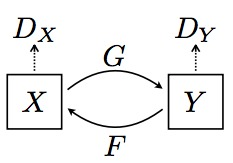
\includegraphics[width=.35\textwidth]{cyclegan_1}
    \label{cyclegan_1}
    \caption{}
\end{figure}

CycleGAN将对抗损失应用到了两个映射函数上,对于映射函数$G:X\to Y$和他的判别器$D_Y$,可以将其目标函数表示为
\begin{align*}
    \label{eq:2}
    \centering
    L_{GAN}(G,D_Y,X,Y)= & \xi_{y\sim p_{data}(y)}[\log D_Y(y)] + \\
    & \xi_{x\sim p_{data}(x)}[\log (1-D_Y(G(x)))]
\end{align*}

这里的$G$试图产生类似于类$Y$的图像集$G(x)$,然而$D_Y$的目标是区分转换的图像$G(x)$和真实的图像数据$y$。$G$旨在与对抗器$D$竞争最小化该目标函数。

对抗器理论上可以训练出可以输出和目标类$Y$与$X$分布完全相同的数据的映射函数$G$和$F$,但是如果网络的体积足够大,可以将相同的输入图片集映射到目标图片类的任意图像子集里。因此,单靠对抗损失函数无法保证学习到了映射函数能将单张输入图片$x_i$映射到理想的输出$y_i$。为了进一步减小可能的映射函数空间,CycleGAN提出循环一致映射函数,即对于来自类$X$的每张图像,对应的图像转换循环应该能够将$x$转换成原始图片,即\textit{向前循环一致}。上述的循环一致损失函数可以表示为:
\begin{align*}
    \label{eq:3}
    \centering
    L_{cyc}(G,F)= & \xi_{x\sim p_{data}(x)}[||F(G(x))-x||_1] + \\
    & \xi_{y\sim p_{data}(y)}[||G(F(y))-y||_1]
\end{align*}

综合等式\ref{eq:2}和等式\ref{eq:3}我们可以得到总的目标函数:
\begin{align*}
    \centering
    L(G, F, D_X, D_Y) = & L_{GAN}(G,D_Y, X, Y) \\
    & + L_{GAN}(F,D_X, Y, X) \\
    & + \lambda L_{cyc}(G, F)
\end{align*}
这里的$\lambda$控制着两个目标的相对重要性。下图是我们将CycleGAN运用在我们的数据集上的实验结果样本图。

% TODO: add experiment config
% wc ~ 800

\subsubsection{MUNIT}[MUNIT]

\textbf{MUNIT.}\cite{MUNIT}\quad MUNIT是基于UNIT\cite{UNIT}工作的进一步优化。它提出了一个可以解决多模型图片到图片转换问题的框架。它对于图像转换问题提出了几个假设:图片的潜在空间(latent space)可以被分解成内容空间和样式空间。基于上一个假设又提出了不同域类的图片共享一个类似的内容空间,但样式空间不一致。为了将一张图片转换成目标域类,MUNIT提出可以将图片的内容码与目标域类样式码空间的一个随机样式码重组。这里的内容码代表了在图片转换过程中应该被保留的信息元,而状态码则代表了不包含在输入图片中还剩下的变量元。通过采样不同的状态码,MUNIT模型能够产生多样,多模型的输出。以上严格的数学定义如下:

假定$x_1\in \chi_1$和$x_2\in \chi_2$是来自两个图片域类的图片集,给定来自两个不同边缘分布$p(x_1)$和$p(x_2)$的样本图片集,但不知道联合分布$p(x_1, x_2)$。MUNIT的目的是利用学习到的图片到图片转换模型$p(x_{1\to 2}|x_1)$和$p(x_{2\to 1}|x_2)$来预测两个边缘分布$p(x_1|x_2)$和$p(x_2|x_1)$,这里的$x_{1\to 2}$是由将$x_1$转换成$x_2$产生的一个样本输出。一般来说,$p(x_1|x_2)$和$p(x_2|x_1)$通常是十分复杂且多模型分布,为了简化这两个边缘分布,MUNIT提出了\textit{部分共享潜在空间假设}。即假设每张图片$x_i\in \chi_i$都是由两种码,内容码和样式码,组成,其中内容码$c\in C$由两个类域共享,而样式码$s_i\in S_i$则是每个域类图片所特有的。换句话说,一组来自联合分布的对应的图片$(x_1, x_2)$

\subsection{图像风格转换大类}[Neural Style Transfer Class]

\chapter{发现}[Findings]

\chapter{相关研究}[Related Work]

\chapter{总结}[Conclusions]
%\include{body/introduction}

\backmatter
%硕博书序
% !Mode:: "TeX:UTF-8" 
\begin{conclusions}

本文主要针对自动驾驶系统的测试用例,即路况图片的合成技术,围绕对抗生成网络和图像转换技术展开的实证研究。
经过对大量的深度学习模型实验与模型排除后,最后进行的实验数据统计的模型有8个:MUNIT,CycleGAN,EBGAN,AdaIN Style,Deep Photo Style,Fast Photo Style,Fast Neural Transfer,Texture Nets。

在实验的数据统计与总结中,我们提出了3个模型实验结果的比较指标:模型训练时间、FID值和方向盘拐角差。希望通过这3个指标综合、客观的评价比较出每个模型在路况图片转换中的性能优劣。在最终的实验数据以及我们选择的实验模型范围中来看,图像转换技术大类要由于对抗生成网络大类的模型。我们分析原因主要有有两点:

对抗生成网络的性能对训练数据集很敏感,且对数据集图片质量的要求很高,即需要内容数据集和样式数据集的图片内容结果十分接近。而满足要求的数据集往往需要专门的数据集采集工作,成本较高。而图像转换技术主要是对图像的像素色彩和明暗度做修改,所以对数据集的要求没有对抗生成网络的高,且在我们采集的结果数据中,各项指标数据都要优于对抗生成网络。

其次图像转换技术合成最终的图片中,会尽量保持原图片中的结构内容特征,所以对自动驾驶系统的行为干扰会比较小。

本研究的数据和成果基于文章中展开的研究对各个模型在图像转换性能上对提出的指标展开了定量的分析和比较,希望能对以后从事自动驾驶测试的技术人员,在图像转换技术模型选型上能够给出有价值的参考意见。

\end{conclusions}
   % 结论
\bibliographystyle{hithesis} %如果没有参考文献时候
\bibliography{reference}
\begin{appendix}%附录
% -*-coding: utf-8 -*-
%%%%%%%%%%%%%%%%%%%%%%%%%%%%%%%%%%%%%%%%%%%%%%%%%%%%%%%%%
\chapter{附录}[Appendix]%

%%%%%%%%%%%%%%%%%%%%%%%%%%%%%%%%%%%%%%%%%%%%%%%%%%%%%%%%%
\section{拐角差数据统计表}[Steering Angle Difference Statics]
\begin{figure}[h]
    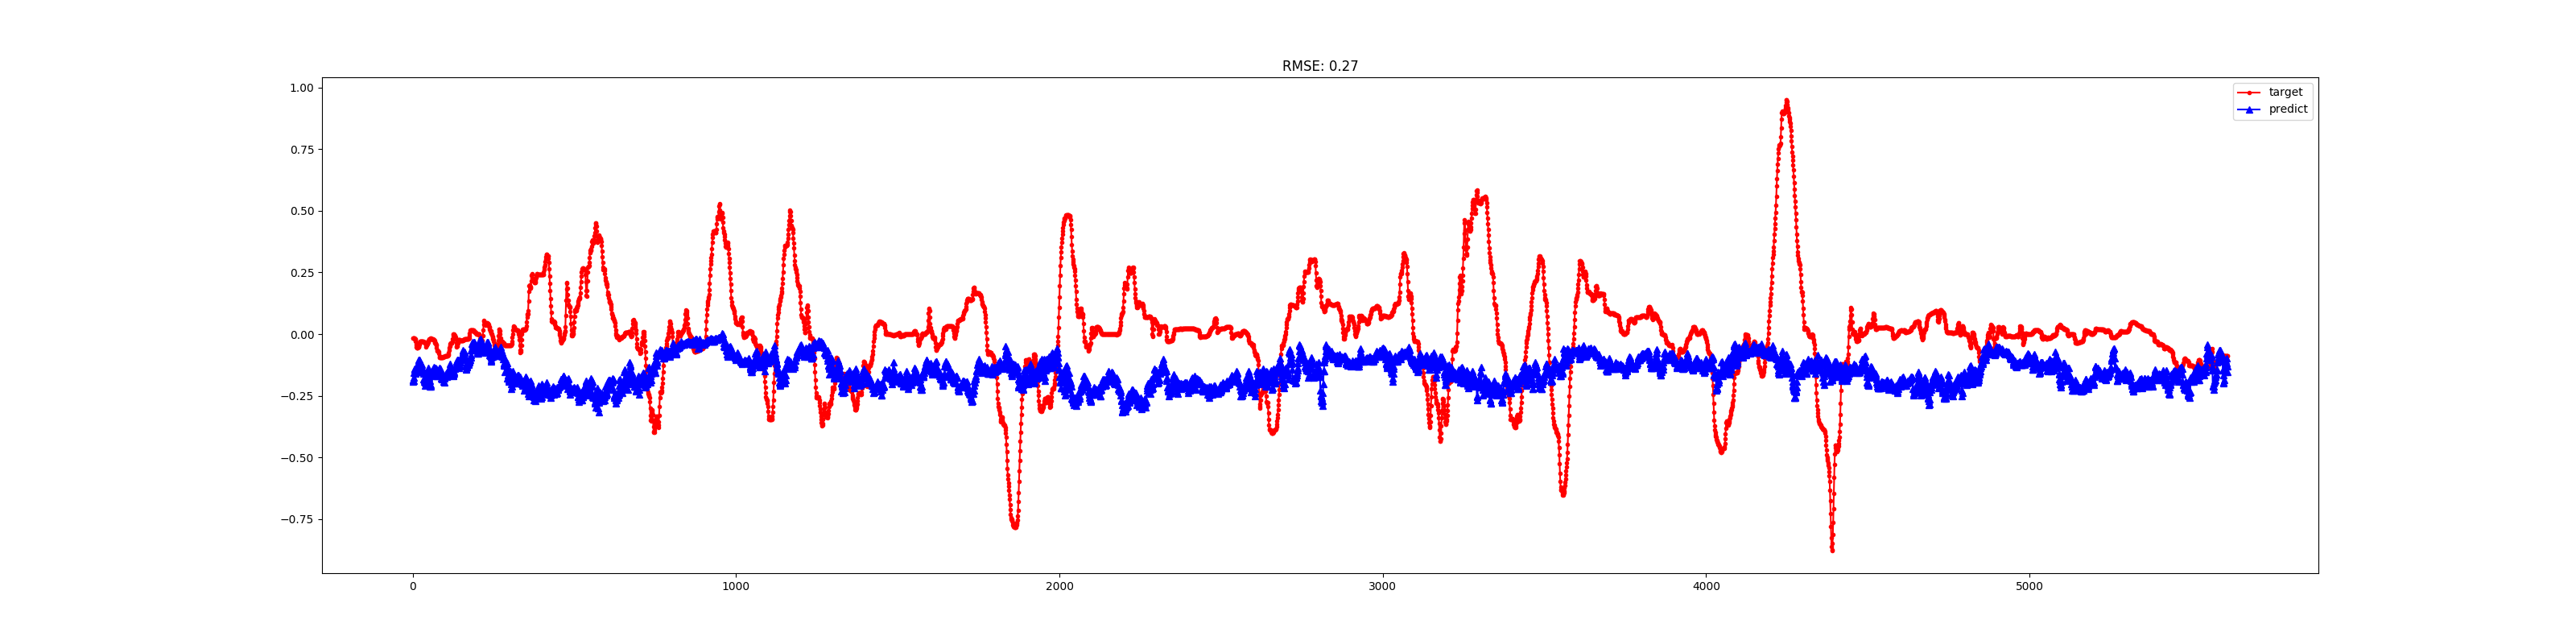
\includegraphics[width=1.5\textwidth, center]{rmse/1} 
    \caption{MUNIT}
\end{figure}
\begin{figure}[h]
    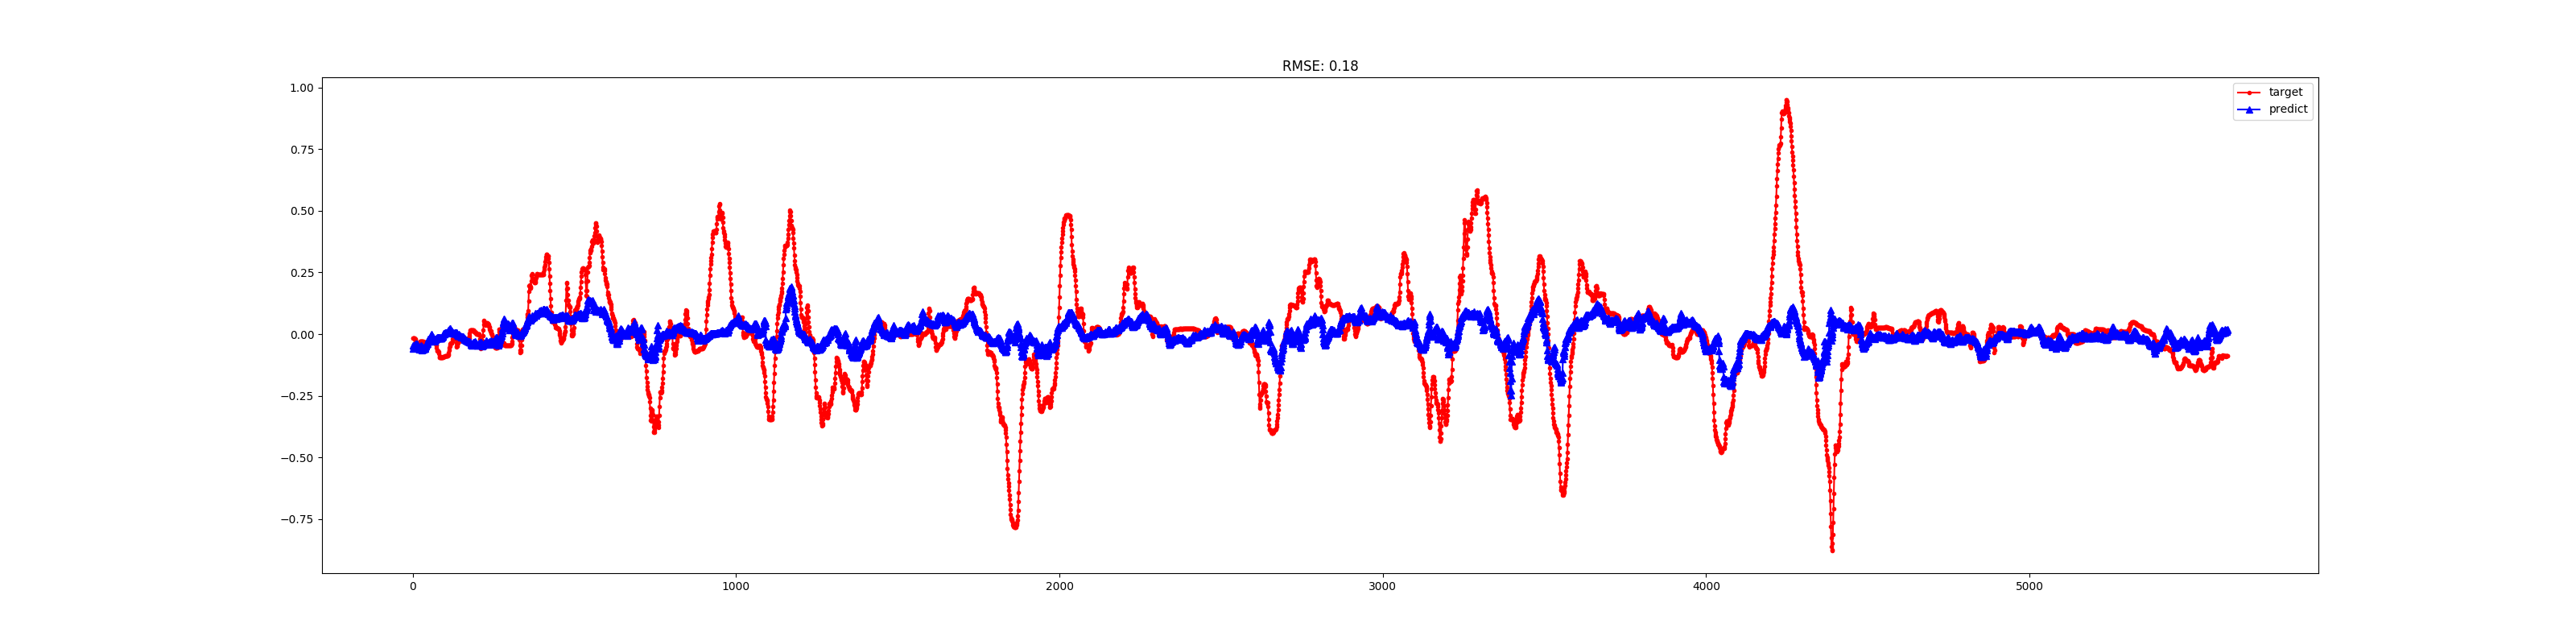
\includegraphics[width=1.5\textwidth, center]{rmse/2} 
    \caption{CycleGAN}
\end{figure}
\begin{figure}[h]
    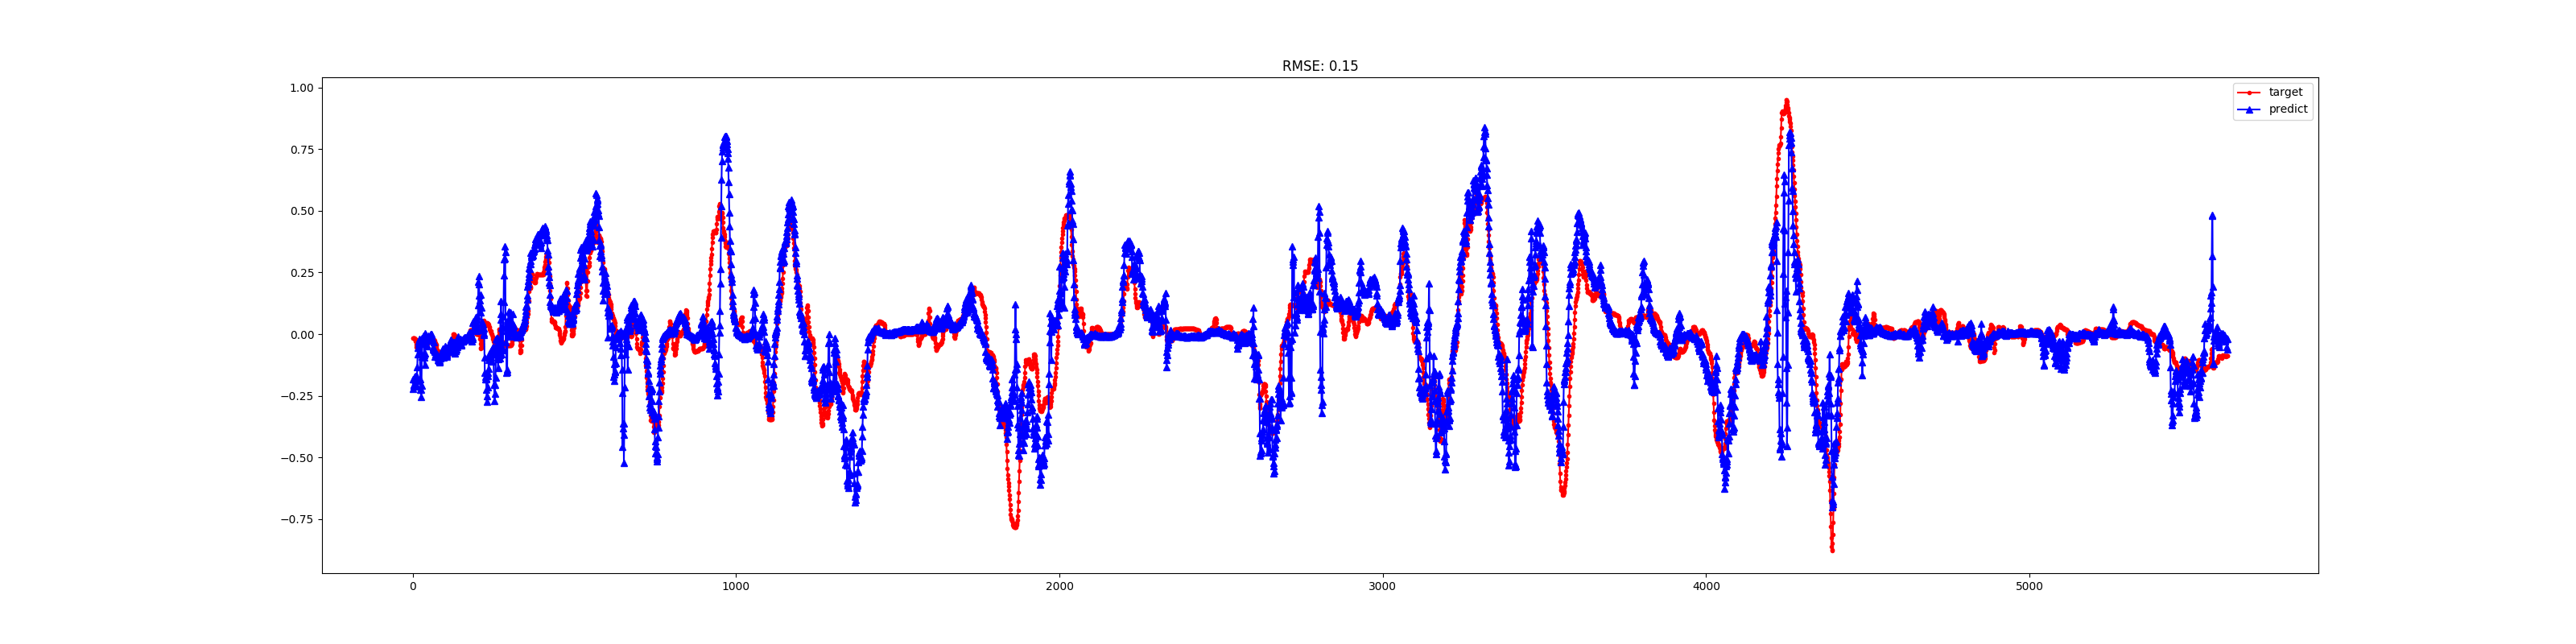
\includegraphics[width=1.5\textwidth, center]{rmse/3} 
    \caption{EBGAN}
\end{figure}
\begin{figure}[h]
    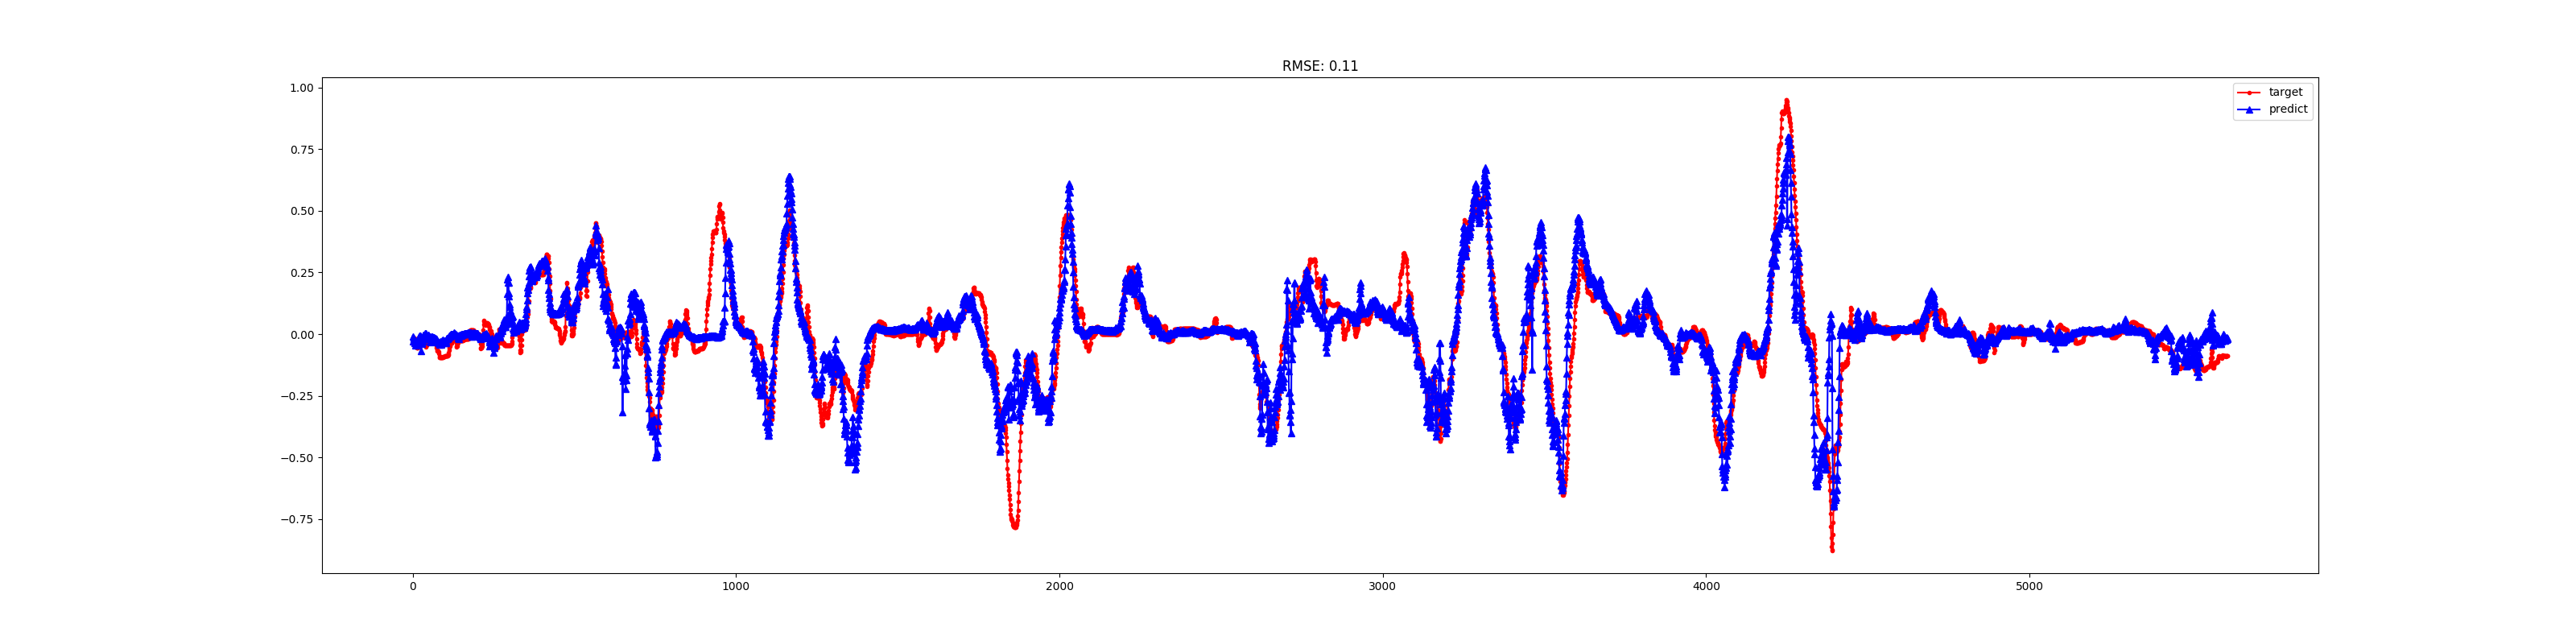
\includegraphics[width=1.5\textwidth, center]{rmse/4} 
    \caption{AdaIN Style}
\end{figure}
\begin{figure}[h]
    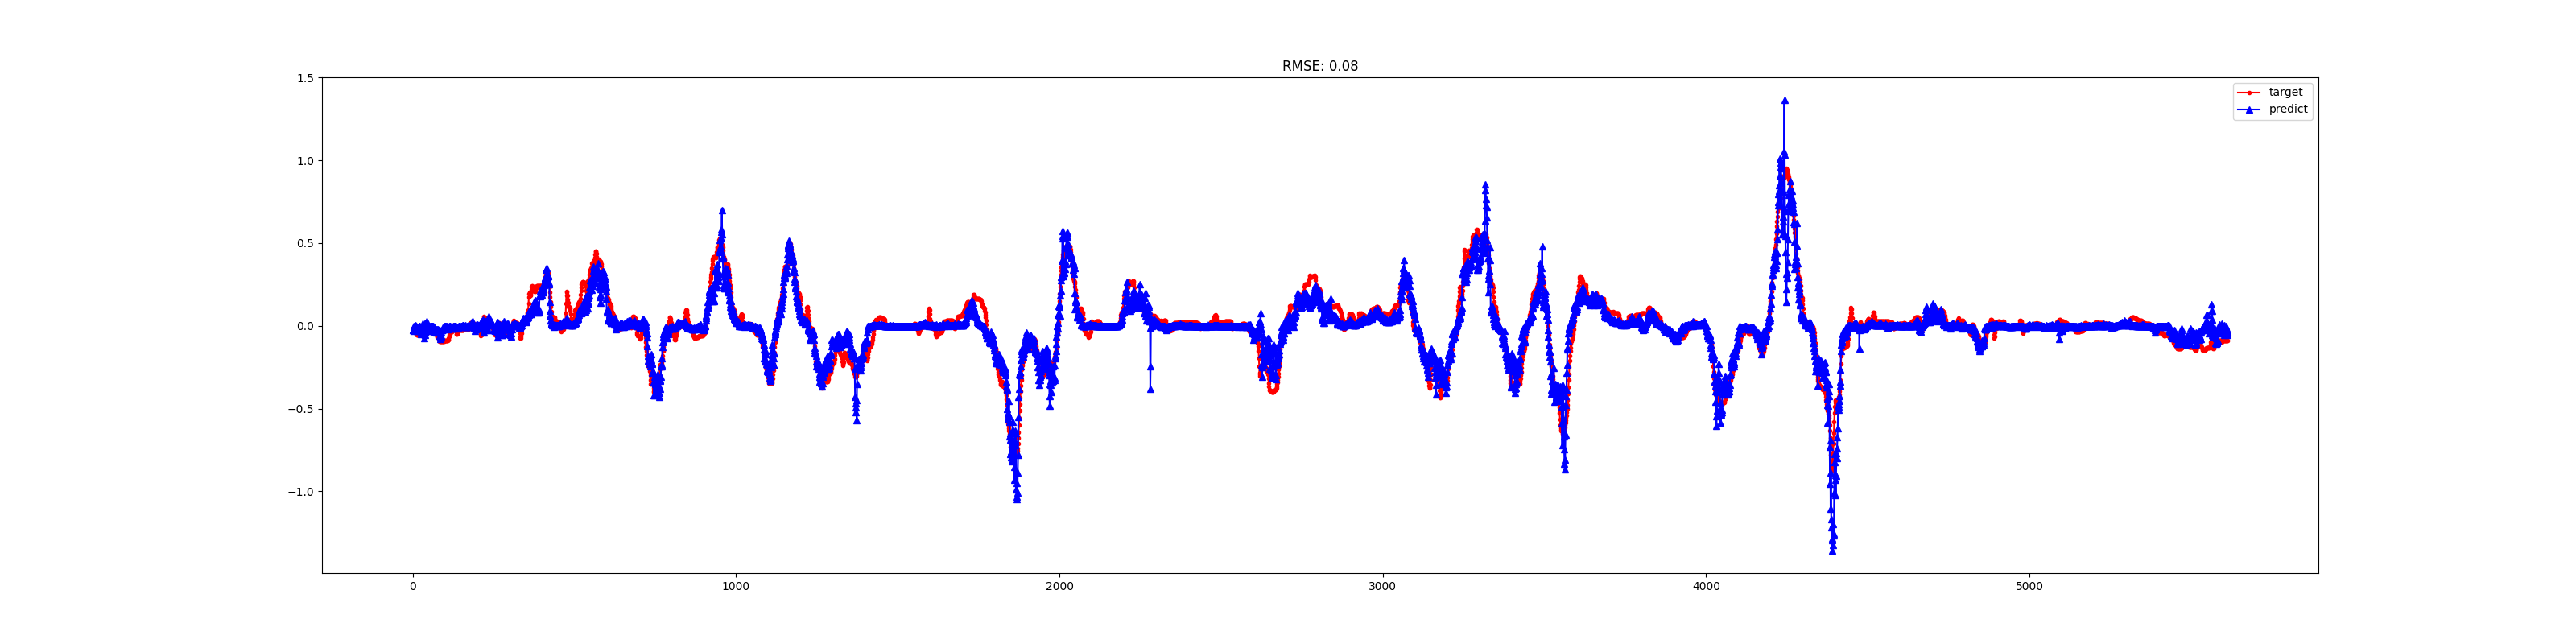
\includegraphics[width=1.5\textwidth, center]{rmse/5} 
    \caption{Deep Photo Style}
\end{figure}
\begin{figure}[h]
    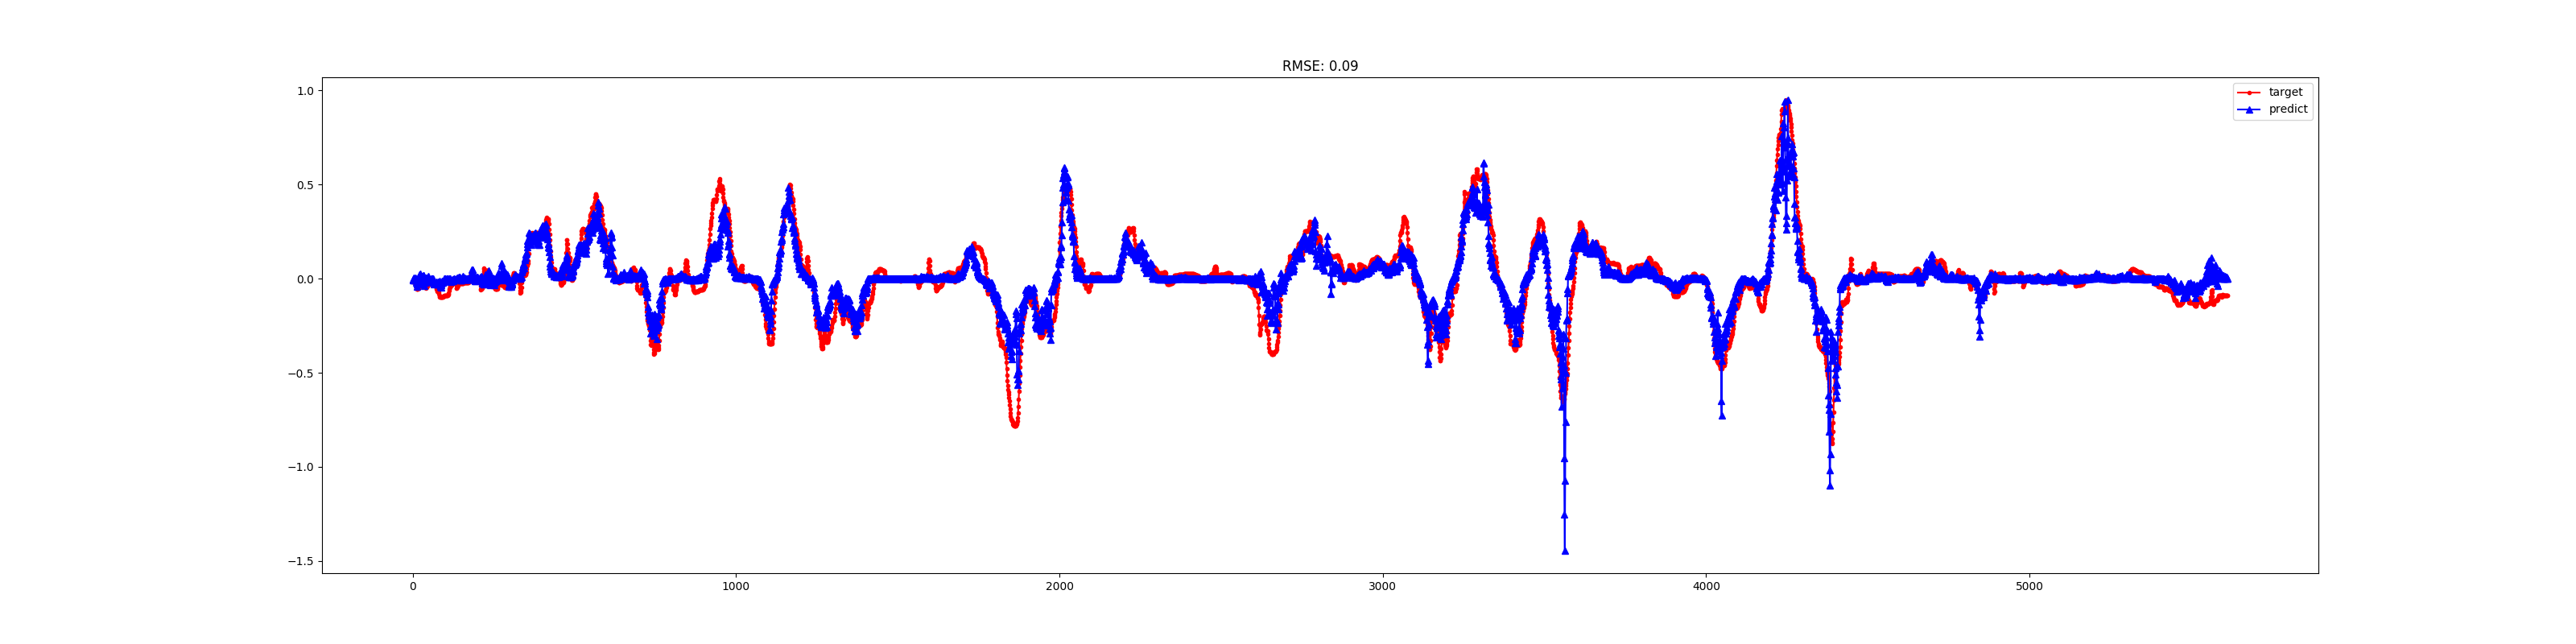
\includegraphics[width=1.5\textwidth, center]{rmse/6} 
    \caption{Fast Photo Style}
\end{figure}
\begin{figure}[h]
    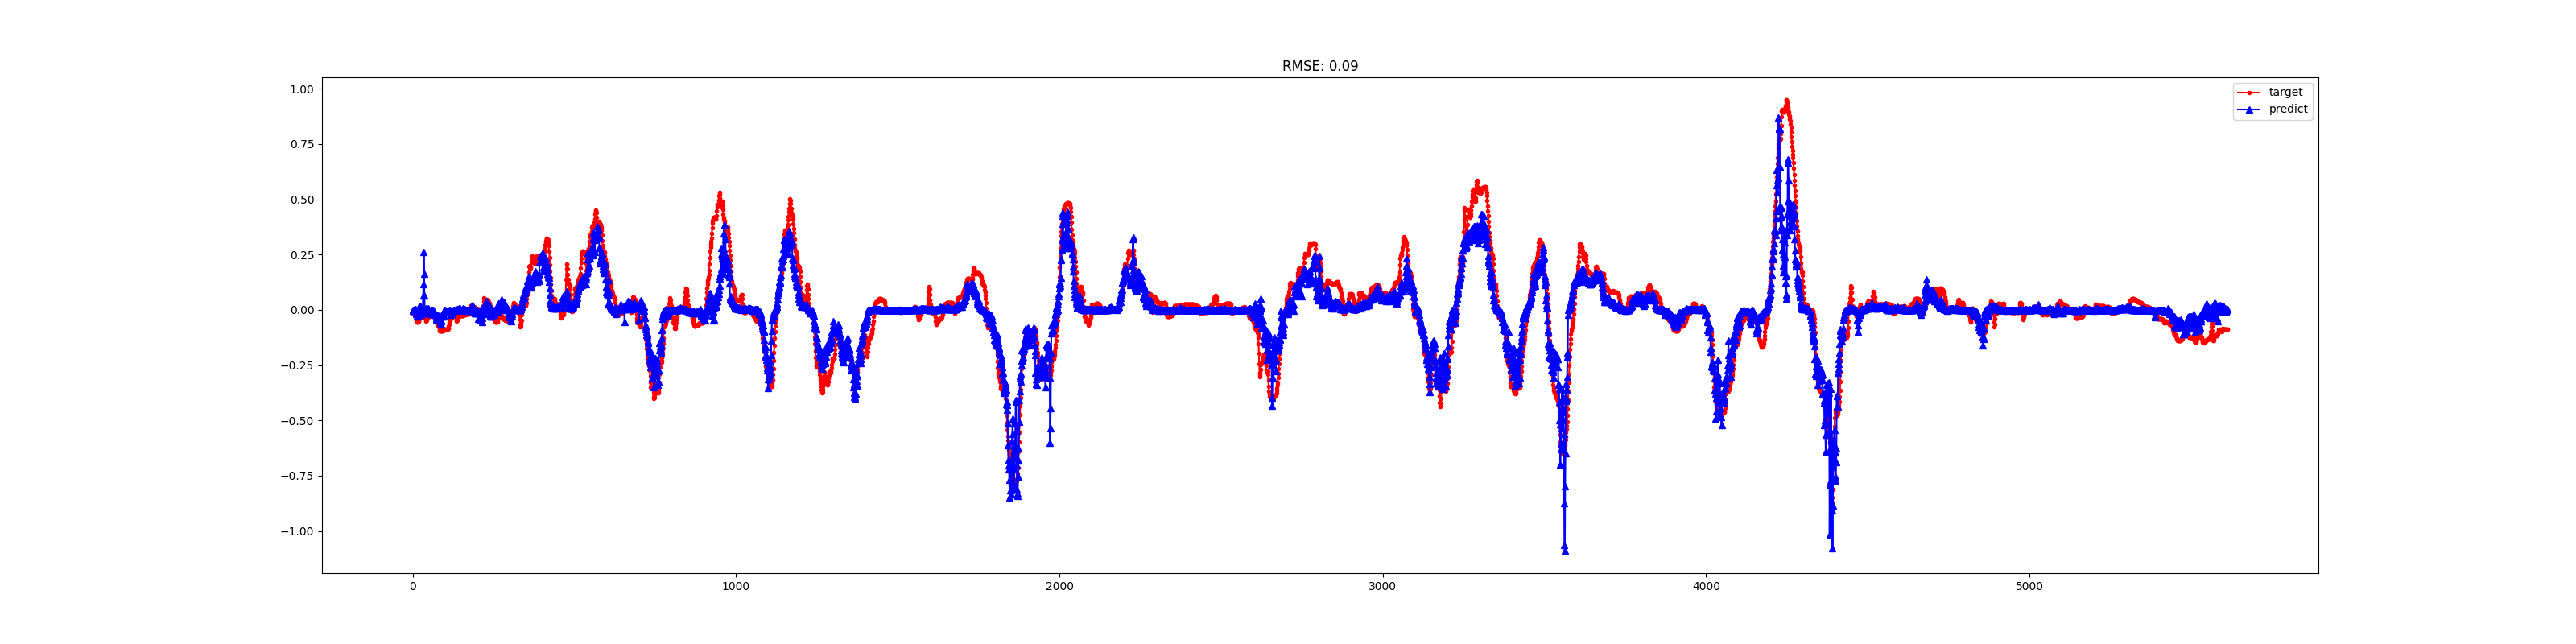
\includegraphics[width=1.5\textwidth, center]{rmse/7} 
    \caption{Fast Neural Transfer}
\end{figure}
\begin{figure}[h]
    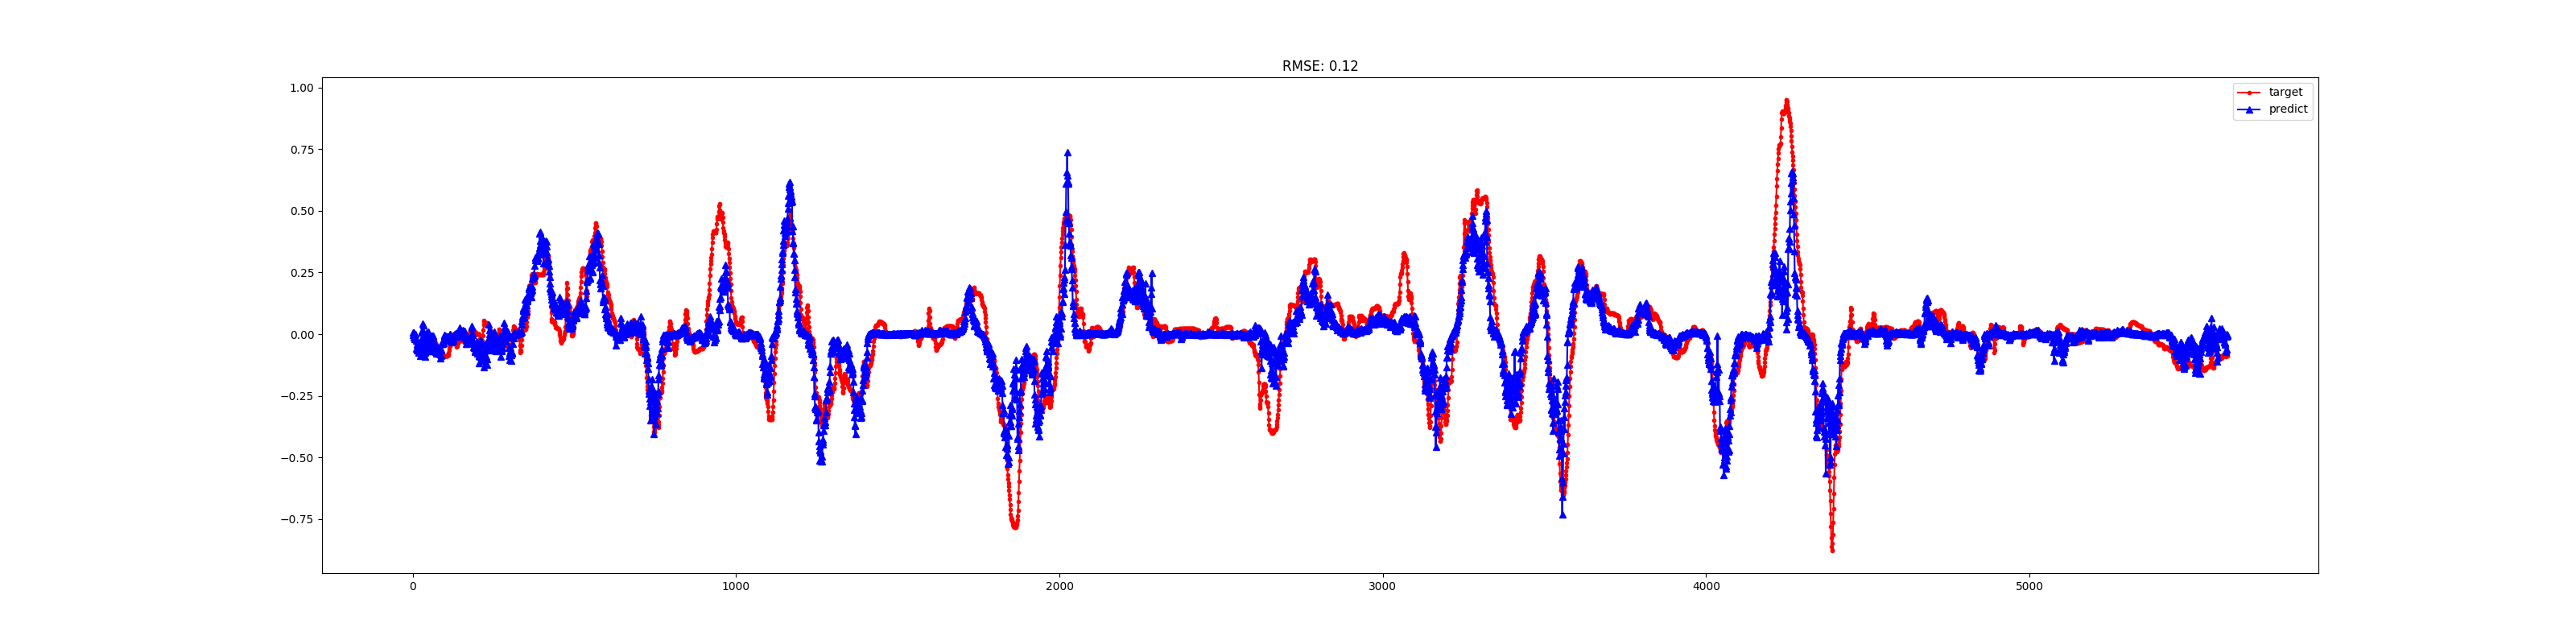
\includegraphics[width=1.5\textwidth, center]{rmse/8} 
    \caption{Texture Nets}
\end{figure}
\end{appendix}
%\include{back/publications}    % 所发文章
\include{back/ceindex}    % 索引, 根据自己的情况添加或者不添加,选择自动添加或者手工添加。
\authorization %授权
%\authorization[saomiao.pdf] %添加扫描页的命令,与上互斥
% !Mode:: "TeX:UTF-8"
\begin{acknowledgements}
衷心感谢导师张煜群教授对本人的精心指导。他的言传身教将使我终生受益。

……

感谢哈工大\LaTeX\ 论文模板\hithesis\ !

\end{acknowledgements}
 %致谢
\include{back/resume}          % 博士学位论文有个人简介

%本科书序为:
%% !Mode:: "TeX:UTF-8" 
\begin{conclusions}

本文主要针对自动驾驶系统的测试用例,即路况图片的合成技术,围绕对抗生成网络和图像转换技术展开的实证研究。
经过对大量的深度学习模型实验与模型排除后,最后进行的实验数据统计的模型有8个:MUNIT,CycleGAN,EBGAN,AdaIN Style,Deep Photo Style,Fast Photo Style,Fast Neural Transfer,Texture Nets。

在实验的数据统计与总结中,我们提出了3个模型实验结果的比较指标:模型训练时间、FID值和方向盘拐角差。希望通过这3个指标综合、客观的评价比较出每个模型在路况图片转换中的性能优劣。在最终的实验数据以及我们选择的实验模型范围中来看,图像转换技术大类要由于对抗生成网络大类的模型。我们分析原因主要有有两点:

对抗生成网络的性能对训练数据集很敏感,且对数据集图片质量的要求很高,即需要内容数据集和样式数据集的图片内容结果十分接近。而满足要求的数据集往往需要专门的数据集采集工作,成本较高。而图像转换技术主要是对图像的像素色彩和明暗度做修改,所以对数据集的要求没有对抗生成网络的高,且在我们采集的结果数据中,各项指标数据都要优于对抗生成网络。

其次图像转换技术合成最终的图片中,会尽量保持原图片中的结构内容特征,所以对自动驾驶系统的行为干扰会比较小。

本研究的数据和成果基于文章中展开的研究对各个模型在图像转换性能上对提出的指标展开了定量的分析和比较,希望能对以后从事自动驾驶测试的技术人员,在图像转换技术模型选型上能够给出有价值的参考意见。

\end{conclusions}
   % 结论
%\bibliographystyle{hithesis}
%\bibliography{reference}
%\authorization %授权
%%\authorization[saomiao.pdf] %添加扫描页的命令,与上互斥
%% !Mode:: "TeX:UTF-8"
\begin{acknowledgements}
衷心感谢导师张煜群教授对本人的精心指导。他的言传身教将使我终生受益。

……

感谢哈工大\LaTeX\ 论文模板\hithesis\ !

\end{acknowledgements}
 %致谢
%\begin{appendix}%附录
%\input{body/appendix01}%本科生翻译论文
%\end{appendix}

\end{document}
